%
%  Contains the appendix for the thesis
%
% For a single appendix, use \makeappendix, and place the
% body of the appendix after it

% For multiple appendices, use \makeappendices, and create each appendix
% using \appendix{}
% For sub-appendices use \appendixsection{} and \appendixsubsection{}

\makeappendices

\renewcommand\thefigure{A.\arabic{figure}}

\appendix{Error by Distribution with a different scale}
\begin{figure}[p]
    \centering
    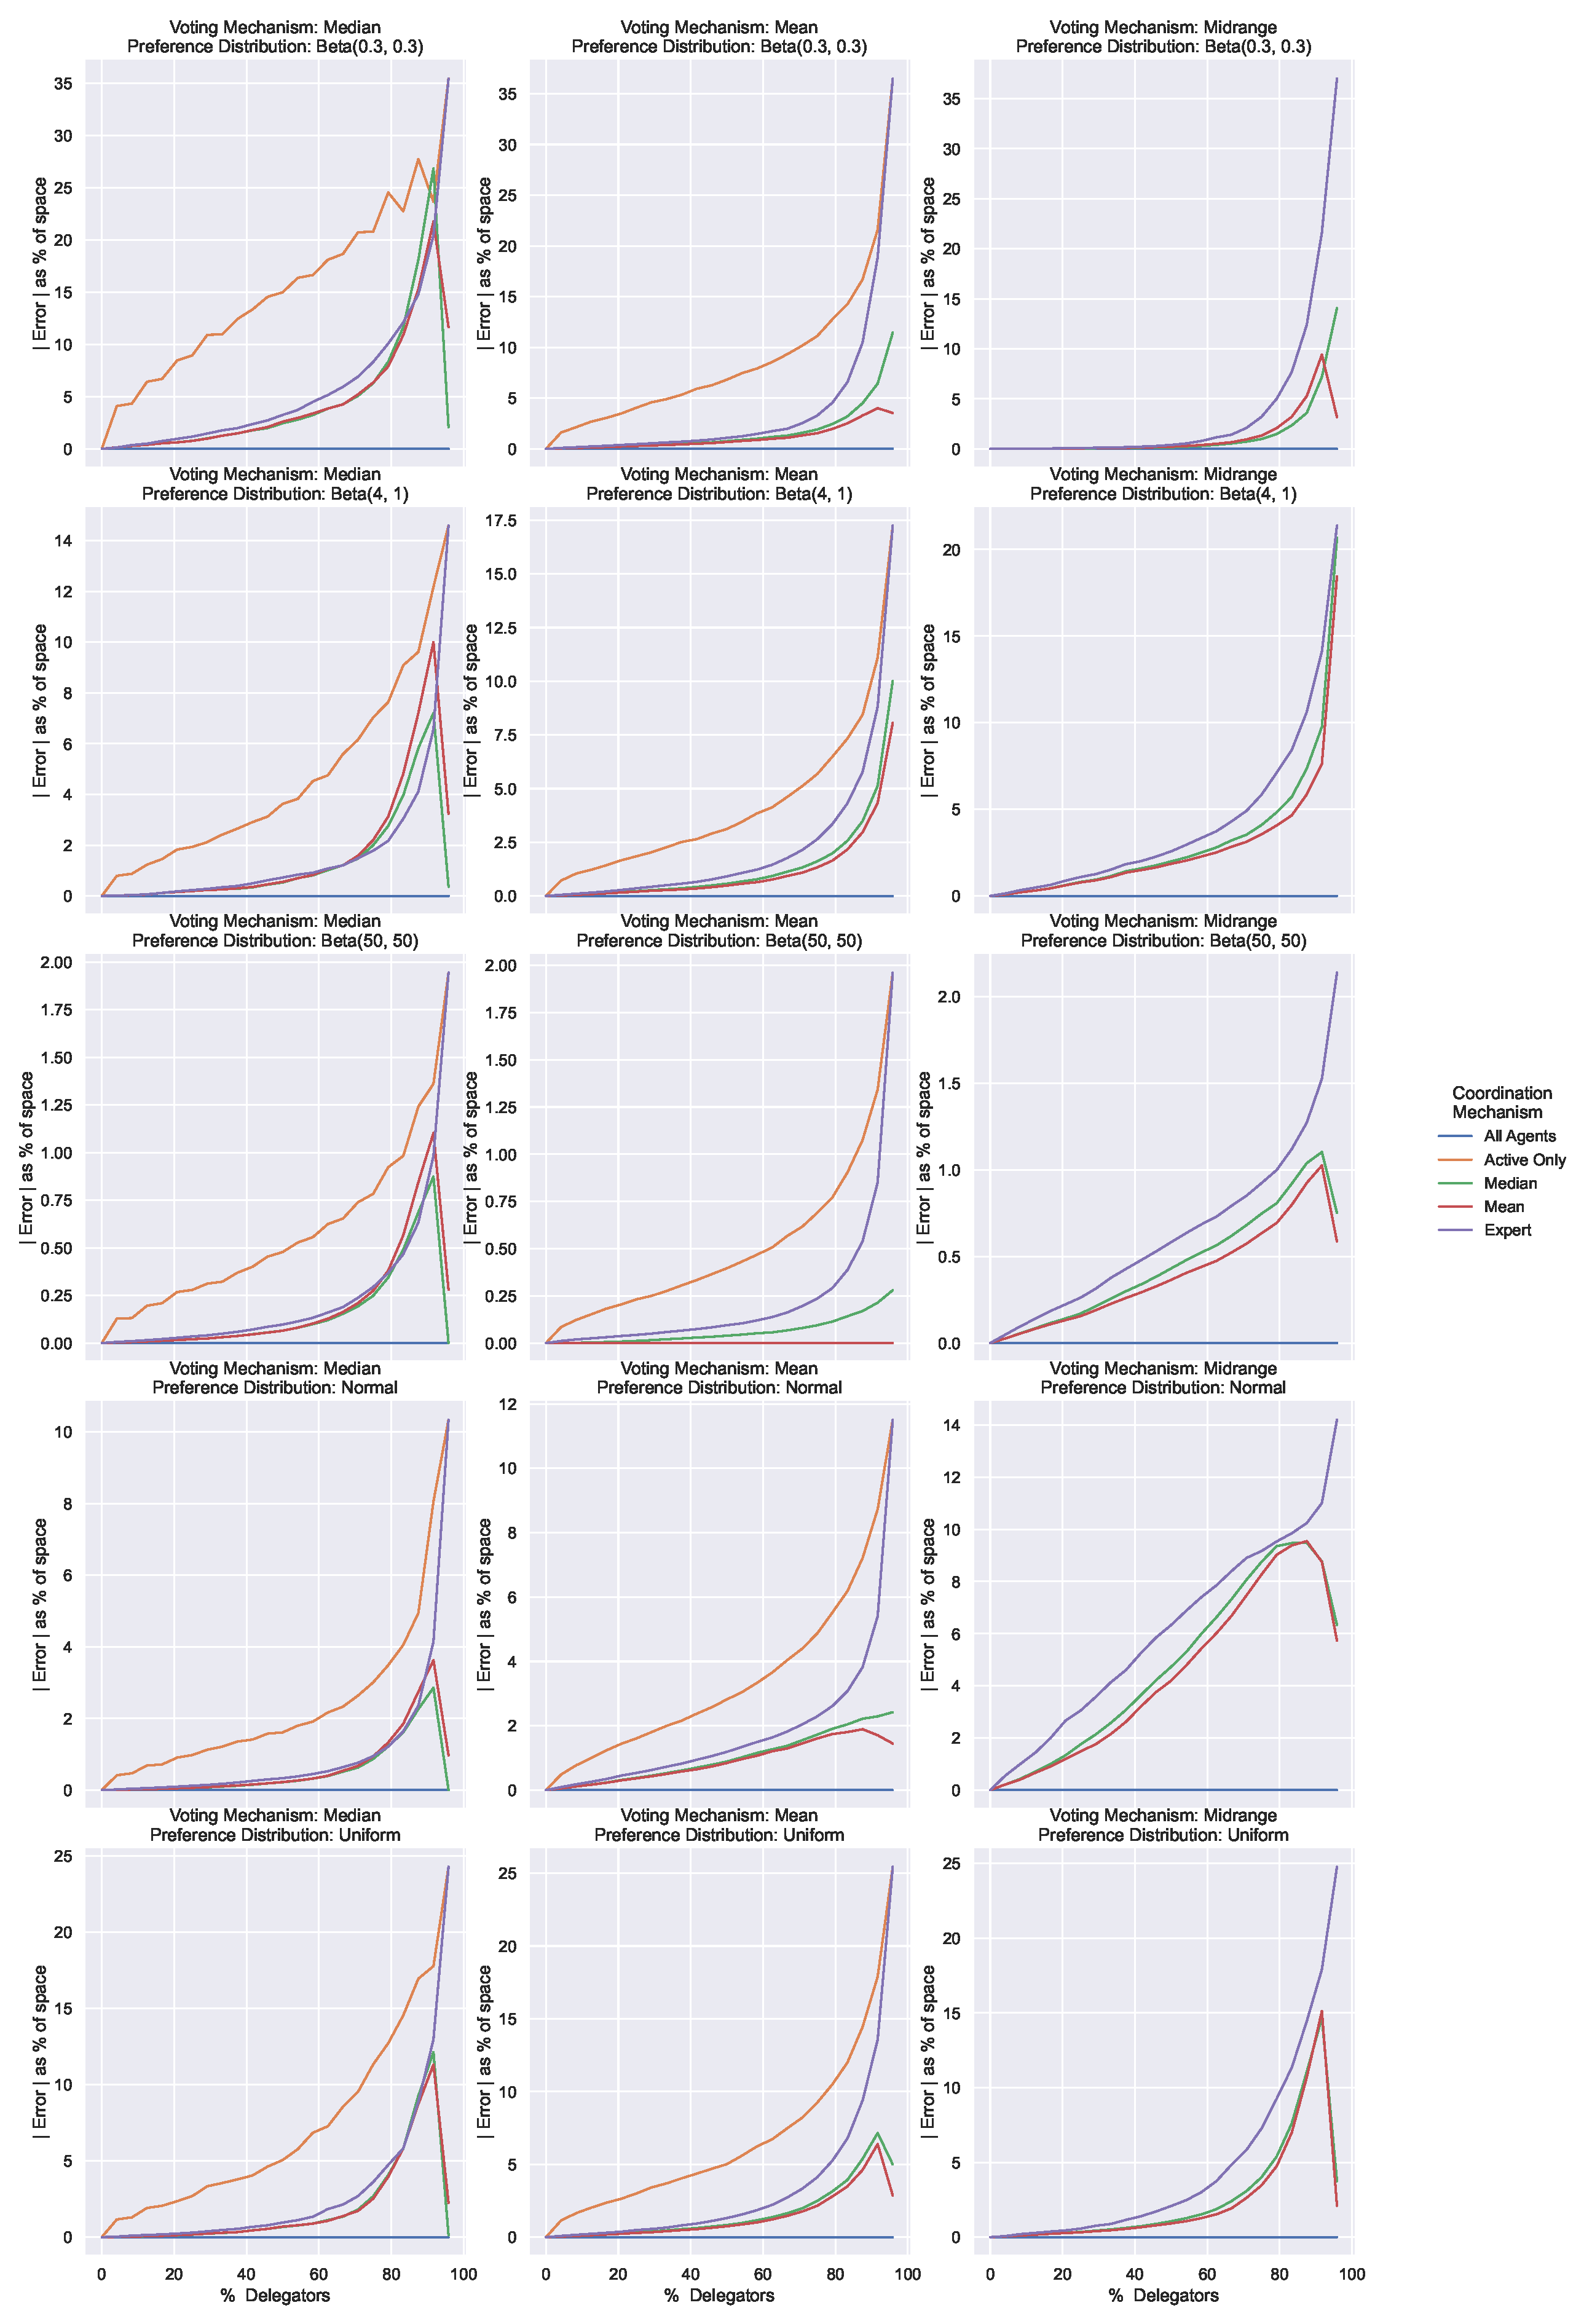
\includegraphics[scale=0.30]
    {content/chapter2/figures/distribution_different_scale_error_as_percent_of_space_abs_mean}
    \caption{
        The absolute error as a percent of the preference space by coordination
        mechanism for each voting mechanism and preference distribution.
        Note the y-axis does not have the same scale for each plot.
        There are 24 total agents.
    }
    \label{fig:distribution-different-scale-error-as-percent-of-space-abs-mean}
\end{figure}

\appendix{Error by Distribution zoomed in}\label{apx:error-by-dist-zoomed}
\begin{landscape}
    \begin{figure}[p]
        \centering
        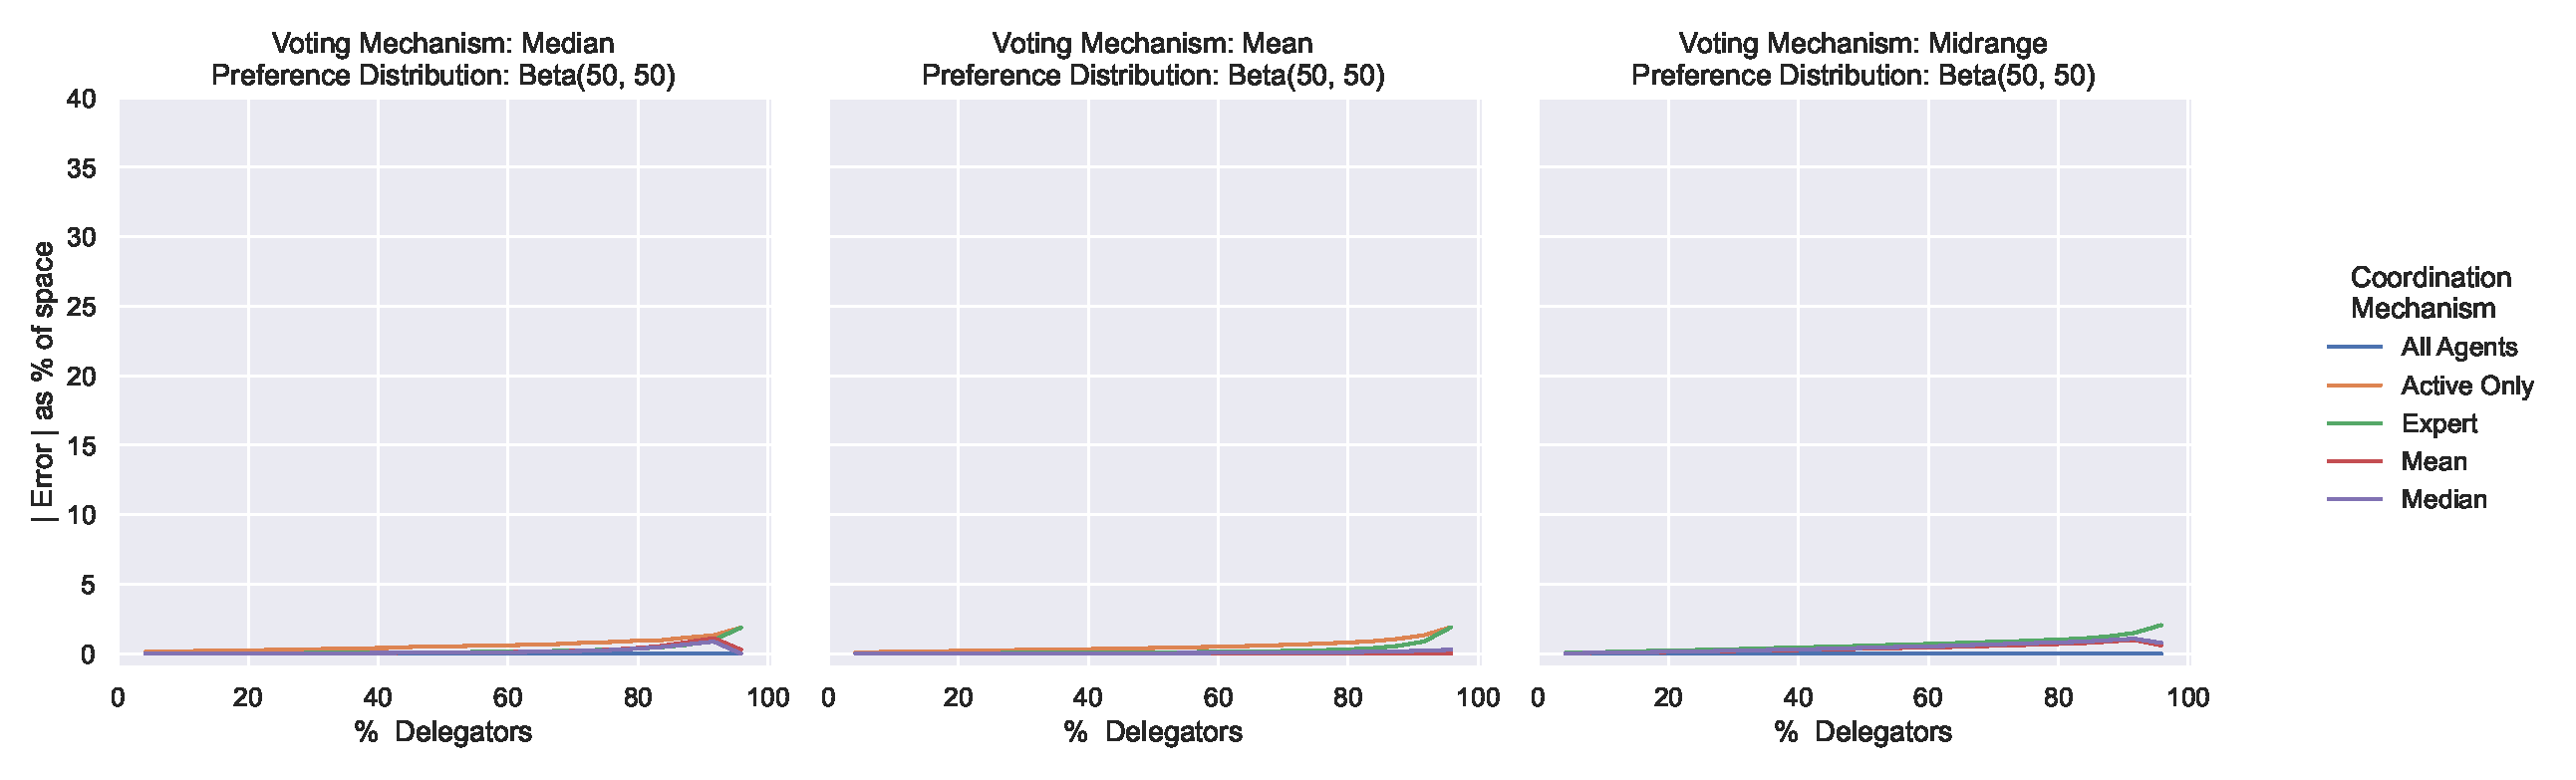
\includegraphics[scale=0.55]
        {content/chapter2/figures/distributions/Beta_50_50_error_as_percent_of_space_abs_mean}
        \caption{
            The absolute error as a percent of the preference space by coordination
            mechanism for each voting mechanism for \betadistribution{50}{50}.
            There are 24 total agents.
        }
        \label{fig:beta-50-50-error-as-percent-of-space-abs-mean}
    \end{figure}
\end{landscape}

\begin{landscape}
    \begin{figure}[p]
        \centering
        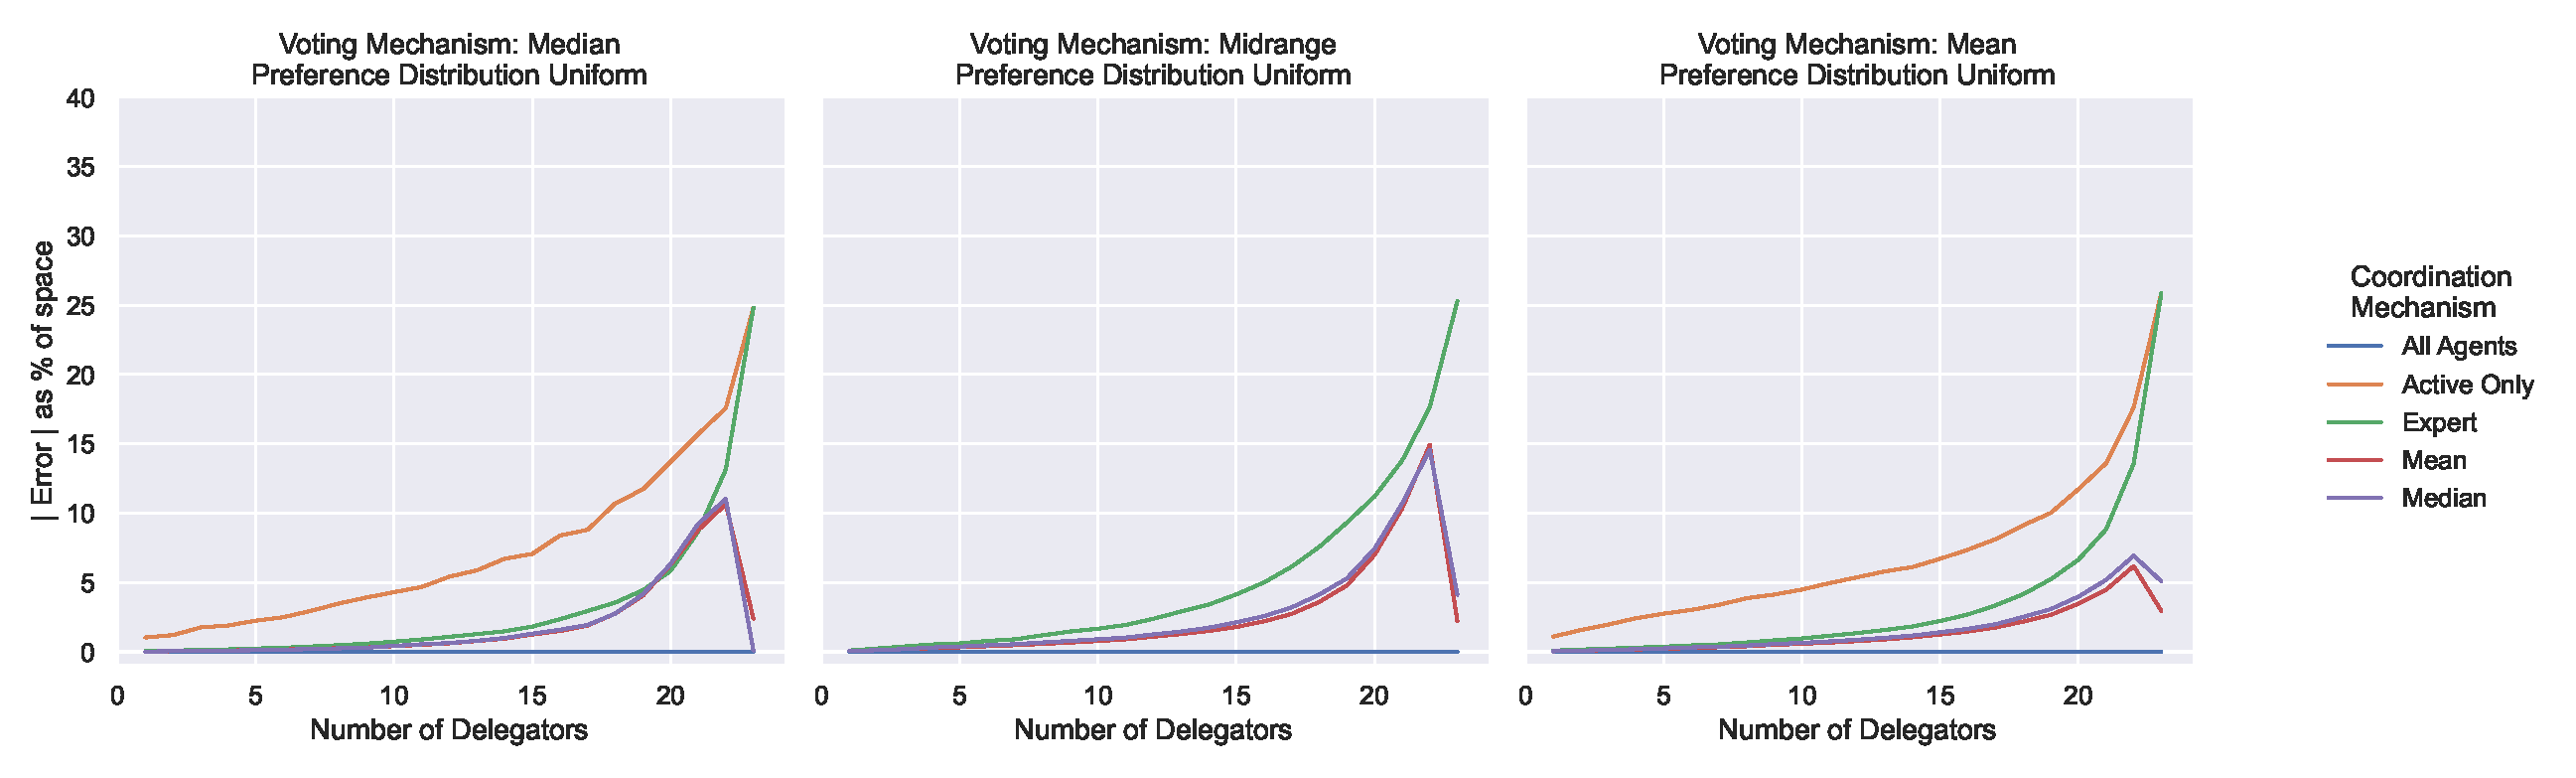
\includegraphics[scale=0.55]
        {content/chapter2/figures/distributions/Uniform_error_as_percent_of_space_abs_mean}
        \caption{
            The absolute error as a percent of the preference space by coordination
            mechanism for each voting mechanism for \uniform{-1}{1}.
            There are 24 total agents.
        }
        \label{fig:uniform-error-as-percent-of-space-abs-mean}
    \end{figure}
\end{landscape}

\begin{landscape}
    \begin{figure}[p]
        \centering
        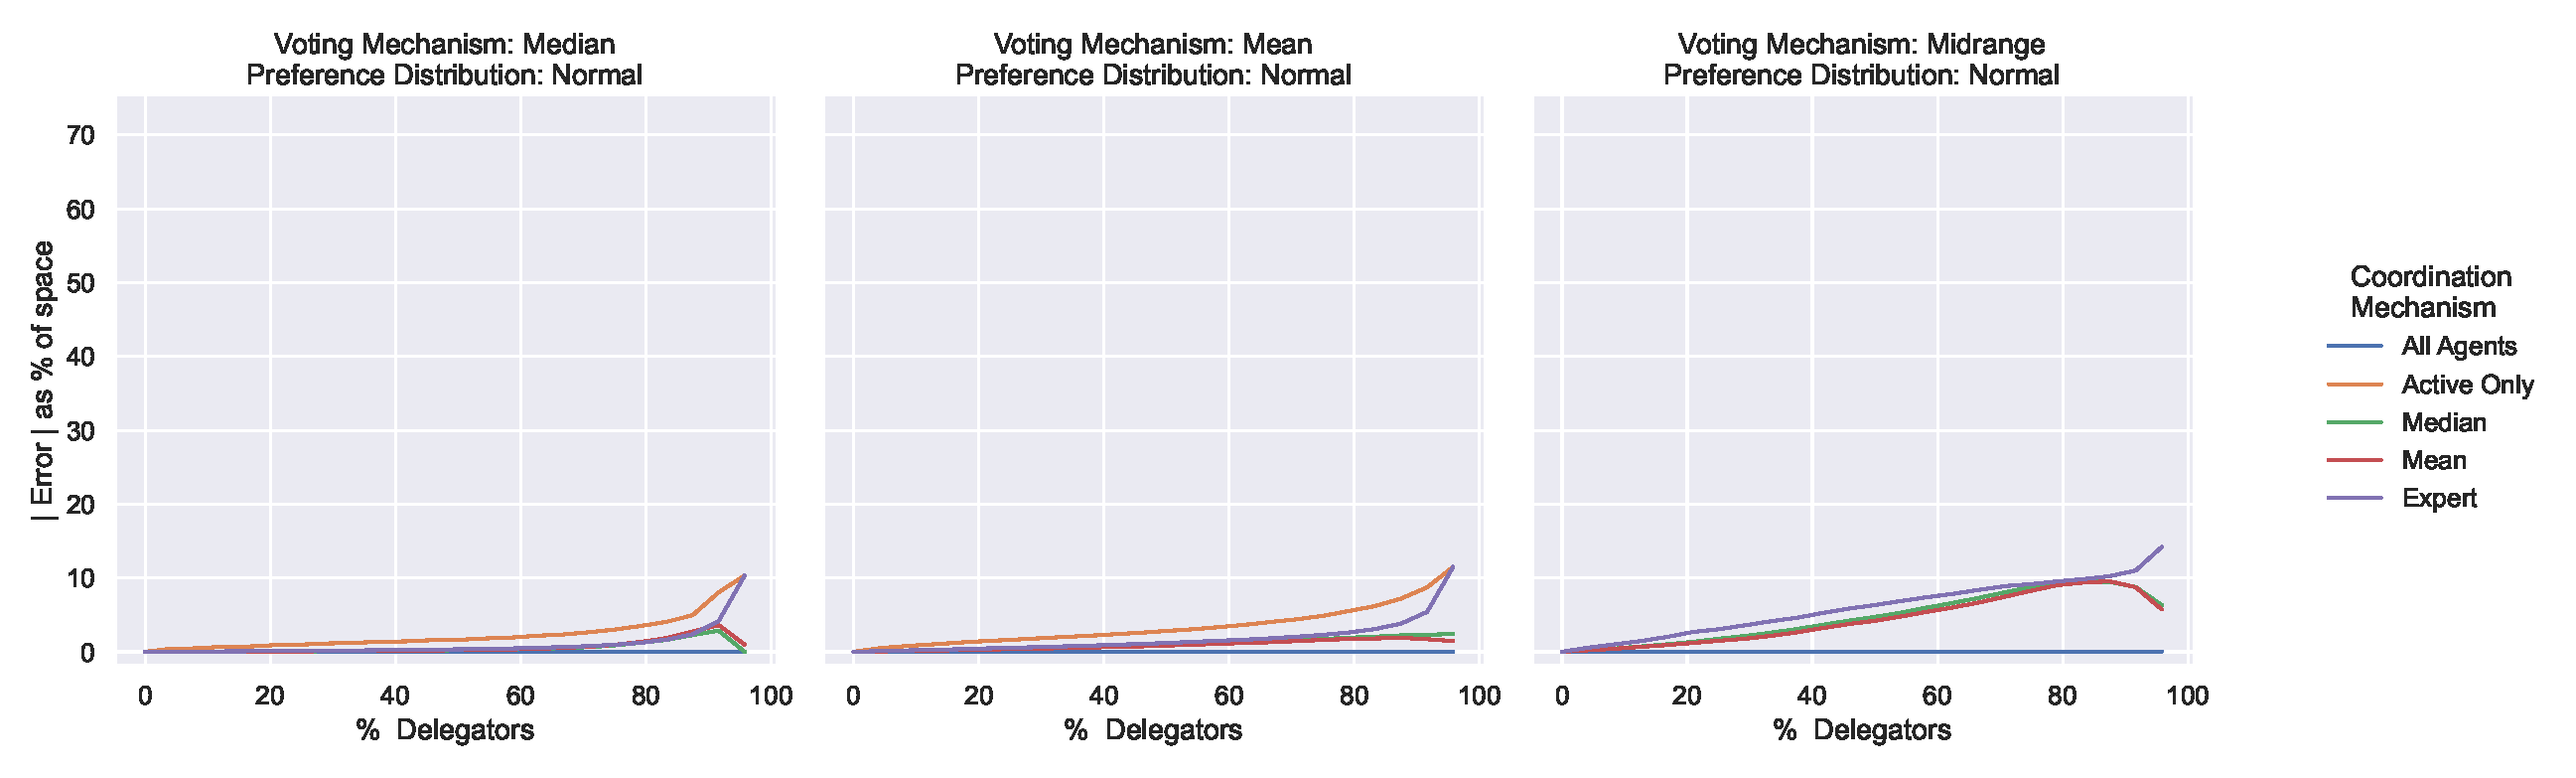
\includegraphics[scale=0.55]
        {content/chapter2/figures/distributions/Normal_error_as_percent_of_space_abs_mean}
        \caption{
            The absolute error as a percent of the preference space by coordination
            mechanism for each voting mechanism for \gaussiandist.
            There are 24 total agents.
        }
        \label{fig:normal-error-as-percent-of-space-abs-mean}
    \end{figure}
\end{landscape}

\begin{landscape}
    \begin{figure}[p]
        \centering
        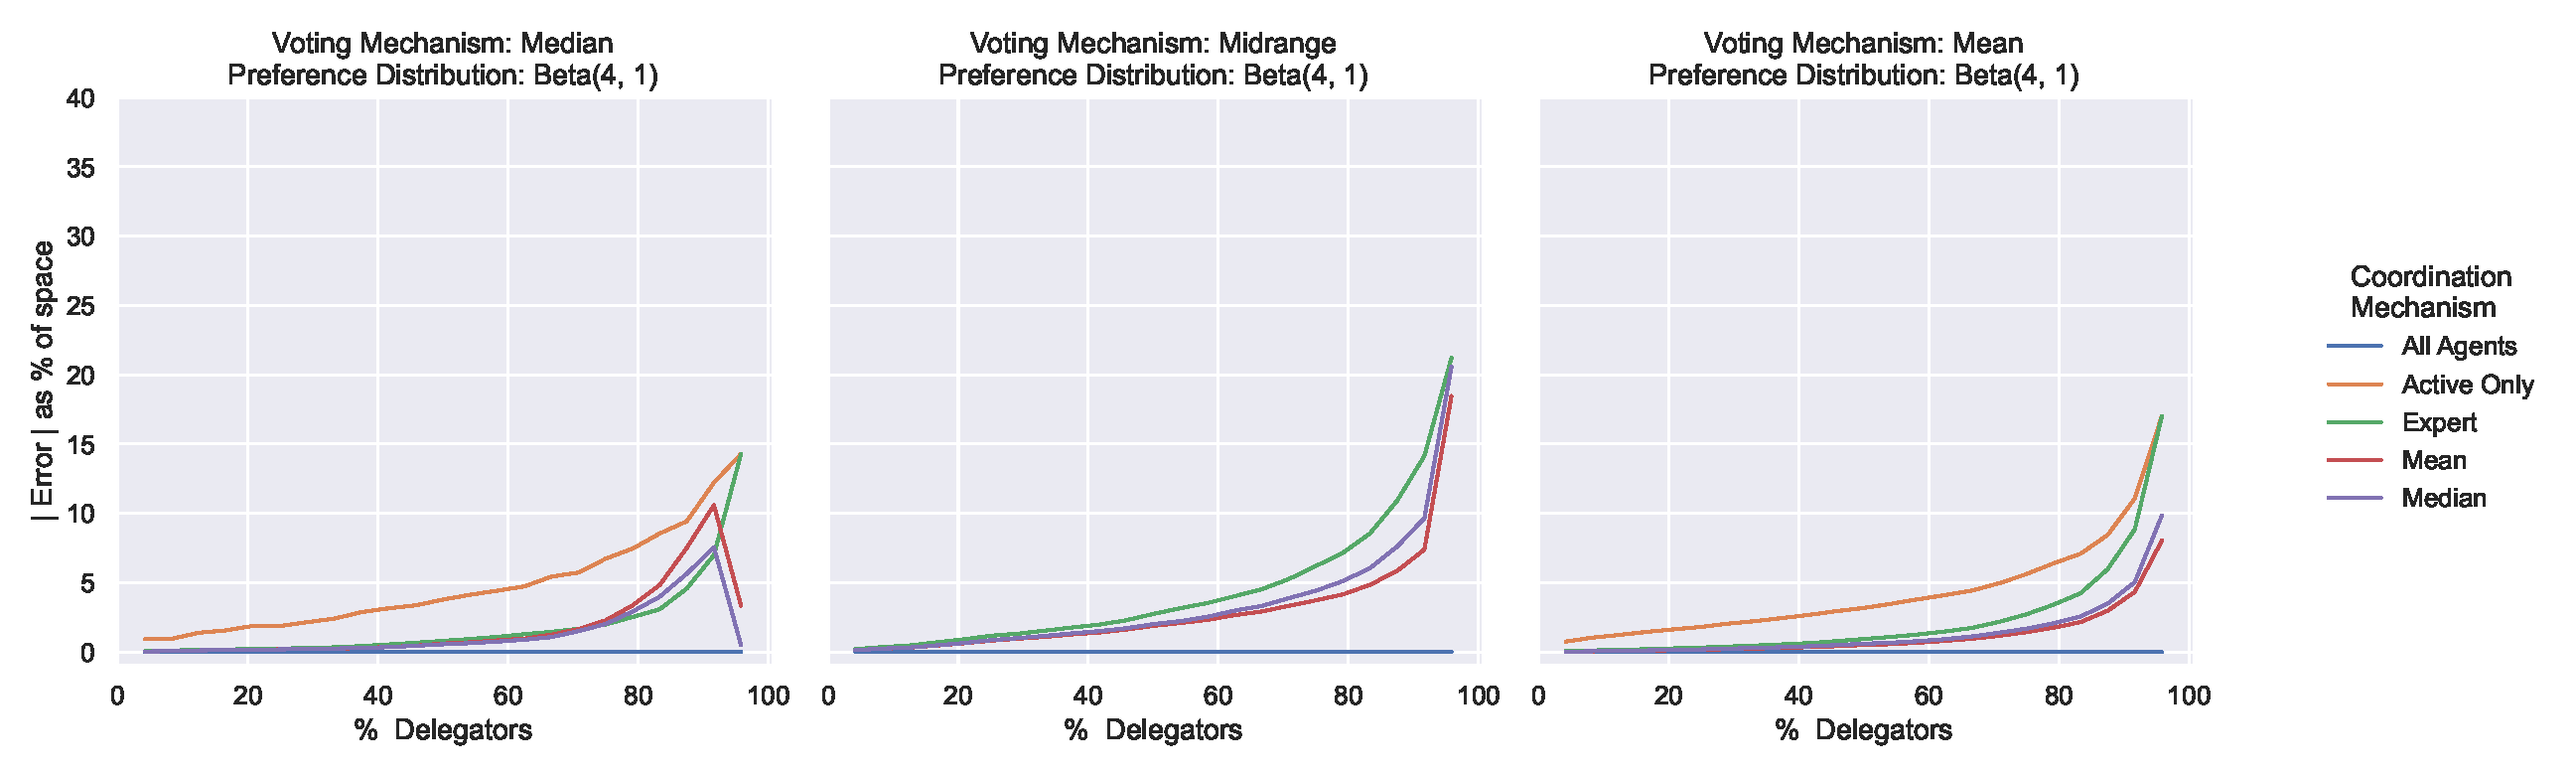
\includegraphics[scale=0.55]
        {content/chapter2/figures/distributions/Beta_4_1_error_as_percent_of_space_abs_mean}
        \caption{
            The absolute error as a percent of the preference space by coordination
            mechanism for each voting mechanism for \betadistribution{4}{1}.
            There are 24 total agents.
        }
        \label{fig:beta-4-1-error-as-percent-of-space-abs-mean}
    \end{figure}
\end{landscape}

\begin{landscape}
    \begin{figure}[p]
        \centering
        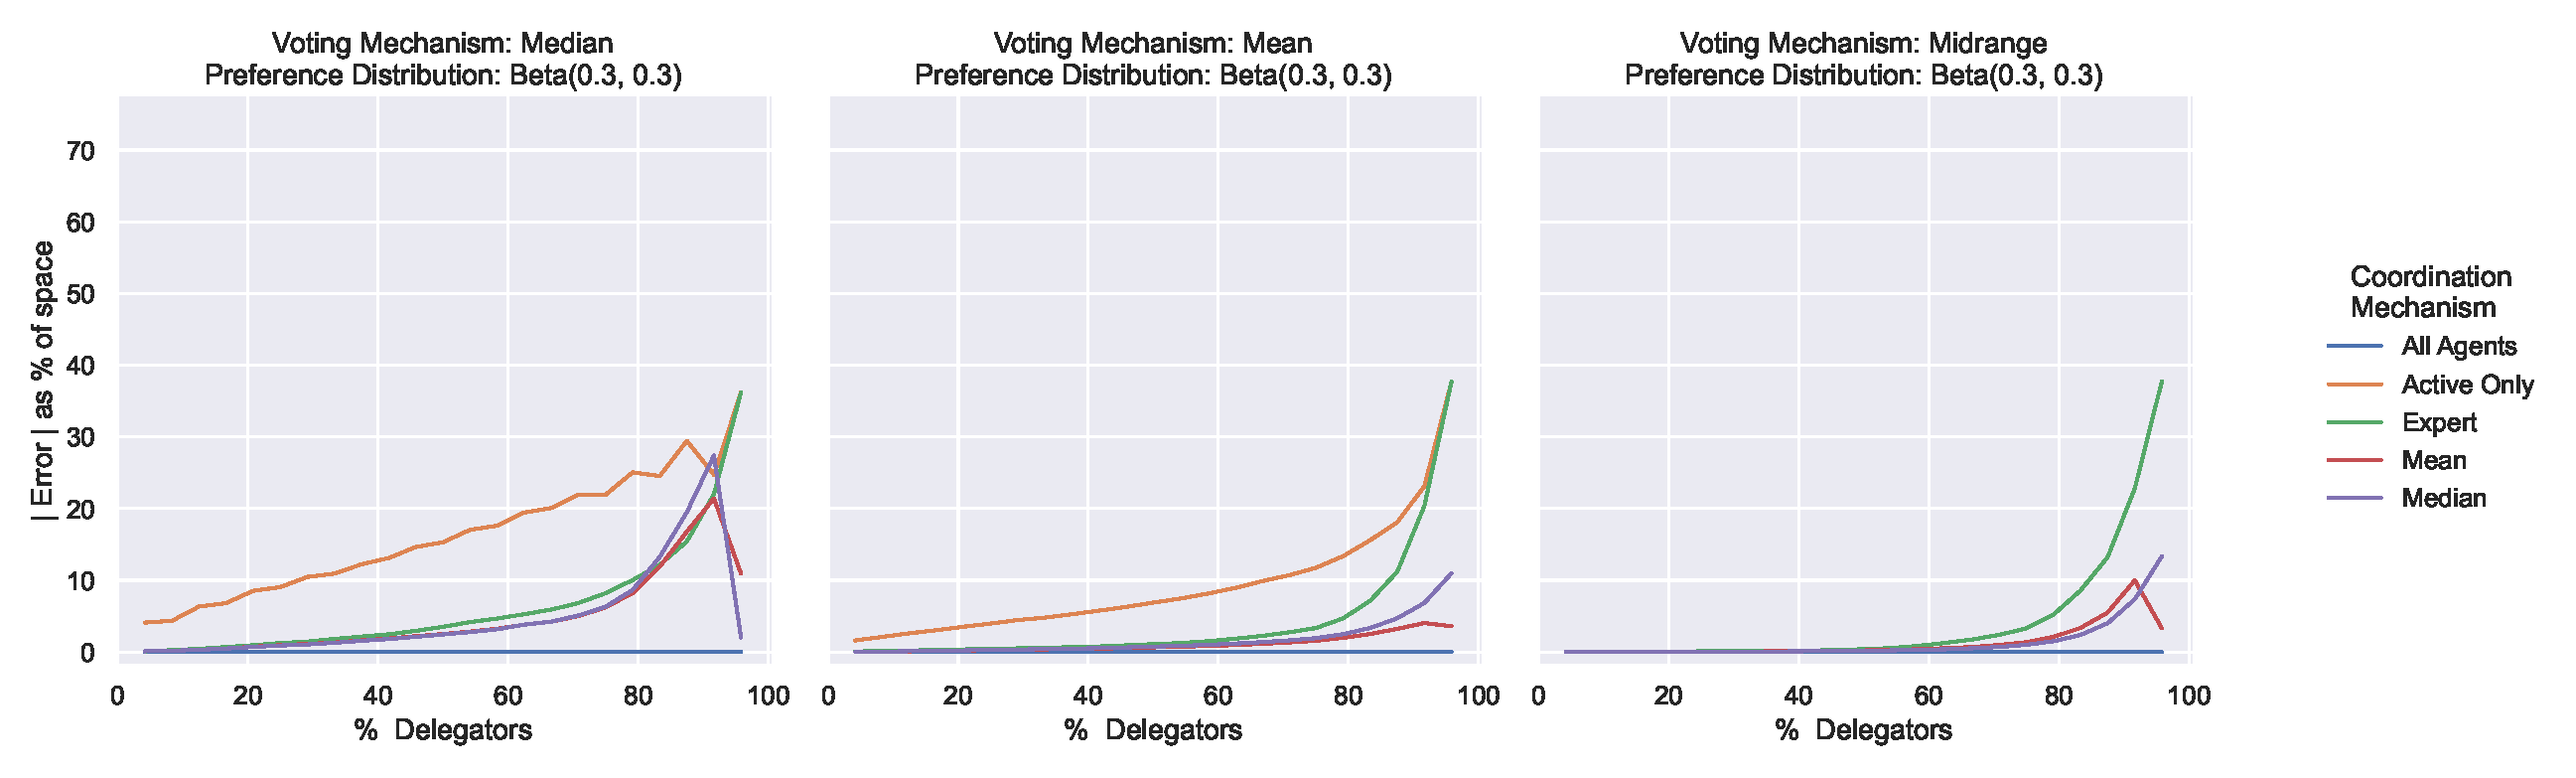
\includegraphics[scale=0.55]
        {content/chapter2/figures/distributions/Beta_0.3_0.3_error_as_percent_of_space_abs_mean}
        \caption{
            The absolute error as a percent of the preference space by coordination
            mechanism for each voting mechanism for \betadistribution{0.3}{0.3}.
            There are 24 total agents.
        }
        \label{fig:beta-.3-.3-error-as-percent-of-space-abs-mean}
    \end{figure}
\end{landscape}